\documentclass[hidelinks,12pt,dvipsnames,border=2pt]{standalone}
%\usepackage[top=0.7in, bottom=0.8in, left=1in, right=1in]{geometry}
\usepackage{tikz}
\usepackage{hyperref}
\usetikzlibrary{arrows}
\usetikzlibrary{shapes}
\usepackage{enumitem}
\usepackage{bm}
\usepackage{mathdots}
\usepackage{amsmath}
\usepackage{tcolorbox}
\usetikzlibrary{shadings}
\usetikzlibrary{decorations.pathreplacing}
\usepackage{helvet}
\usepackage{url}
\usepackage{graphicx}
\usetikzlibrary{arrows.meta,positioning,fit,calc}
\renewcommand{\familydefault}{\sfdefault}


\usetikzlibrary{arrows,decorations.pathmorphing,backgrounds,fit,positioning,shapes.symbols,chains}

\begin{document}
	
% trim=left botm right top
\begin{tikzpicture}
\node at (7,7) {\LARGE \textbf{Histograms of TiTv Distances as a Function of MAF}};

\node at (0,0) {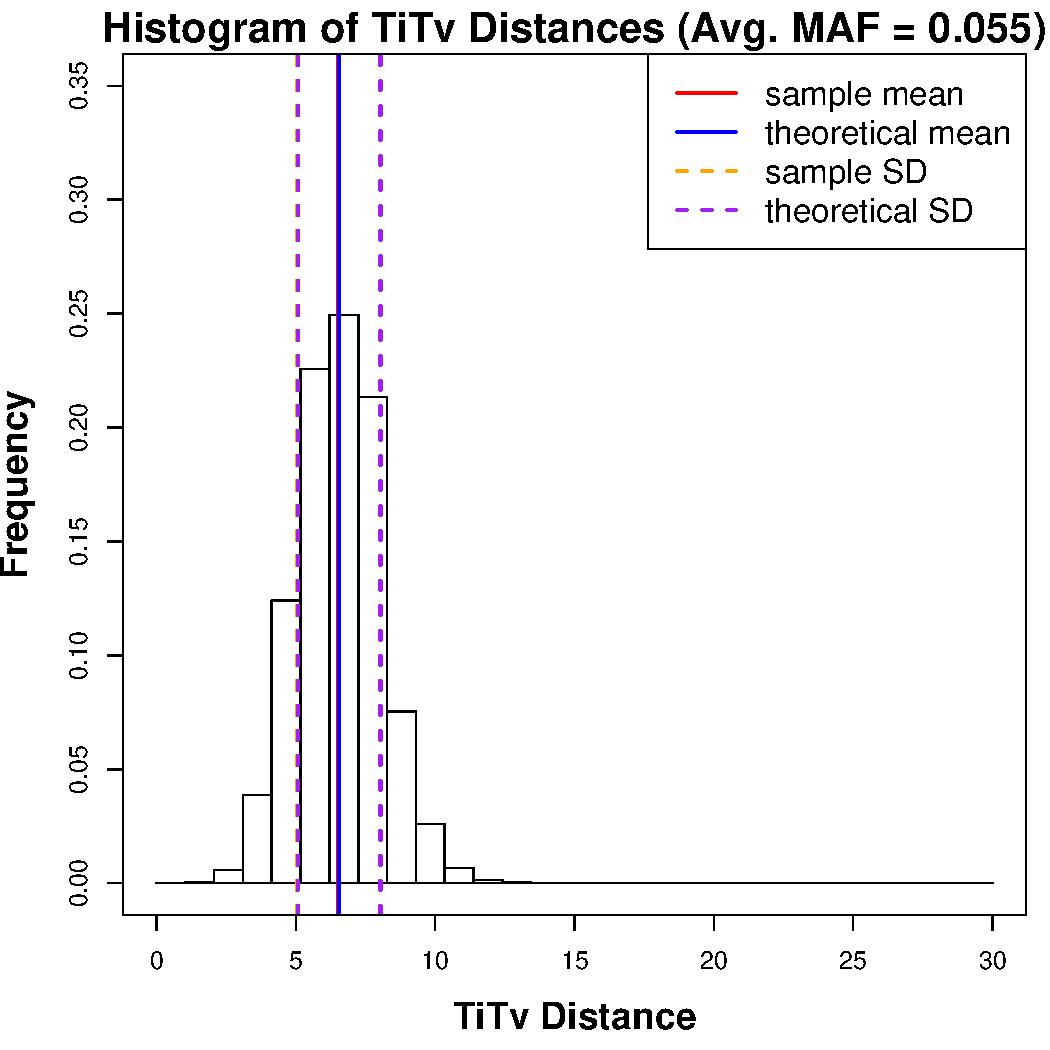
\includegraphics[width=\textwidth]{TiTv_distance_histogram_maf1.pdf}};
\node[fill=black!10,draw=black] at (-2.65,5.97) {\large \textbf{Avg. MAF} \bm{$= 0.055$}};

\node at (13,0) {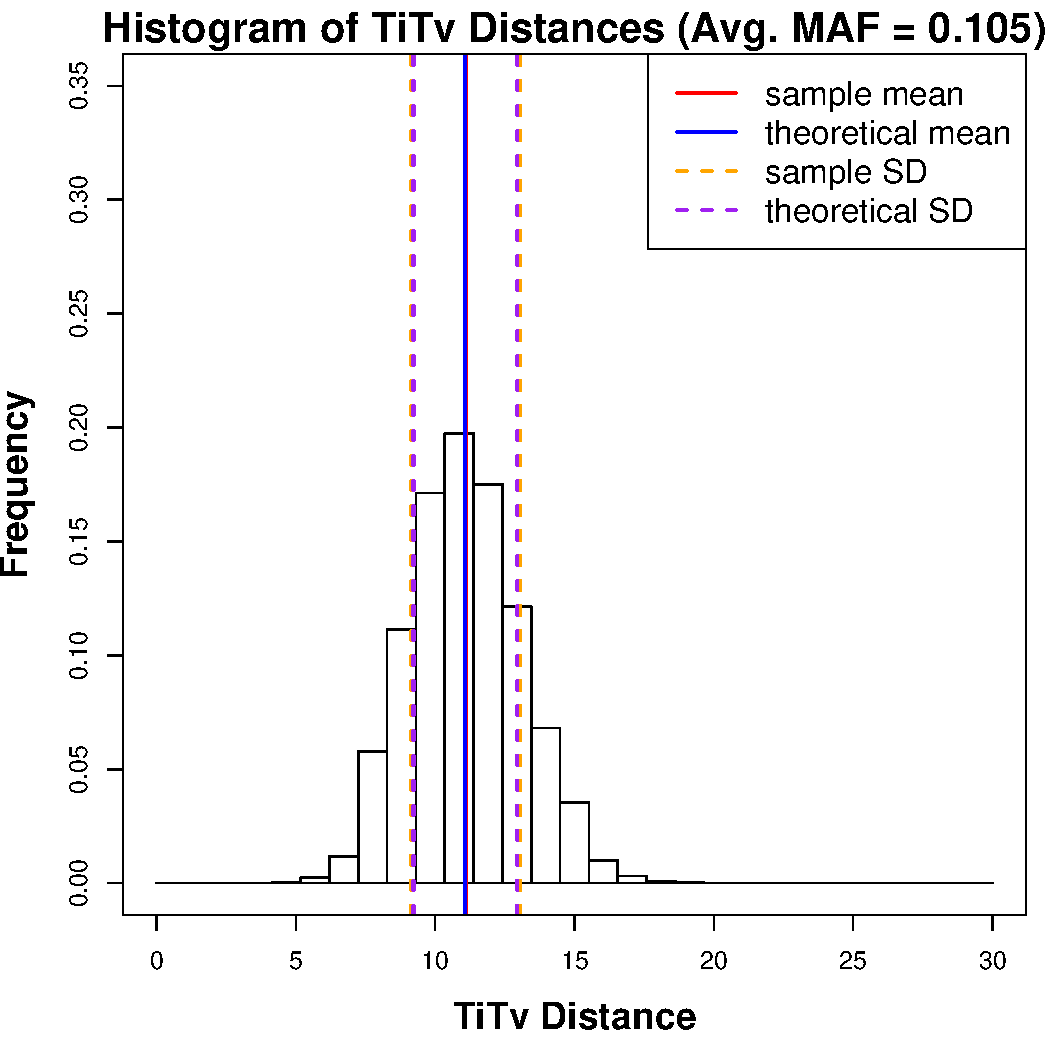
\includegraphics[width=\textwidth]{TiTv_distance_histogram_maf2.pdf}};
\node[fill=black!10,draw=black] at (10.35,5.97) {\large \textbf{Avg. MAF} \bm{$= 0.150$}};

\node at (0,-12.6) {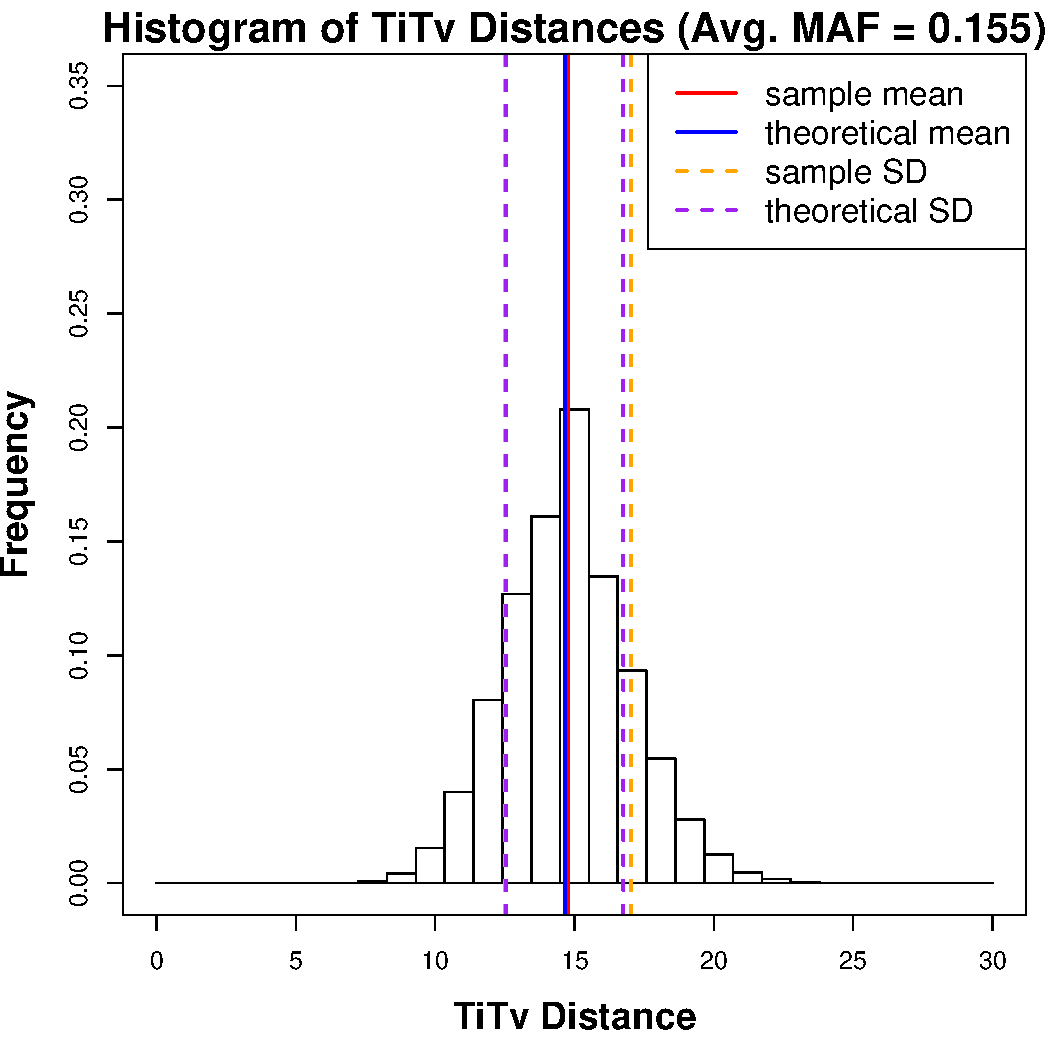
\includegraphics[width=\textwidth]{TiTv_distance_histogram_maf3.pdf}};
\node[fill=black!10,draw=black] at (-2.65,-6.63) {\large \textbf{Avg. MAF} \bm{$= 0.250$}};

\node at (13,-12.6) {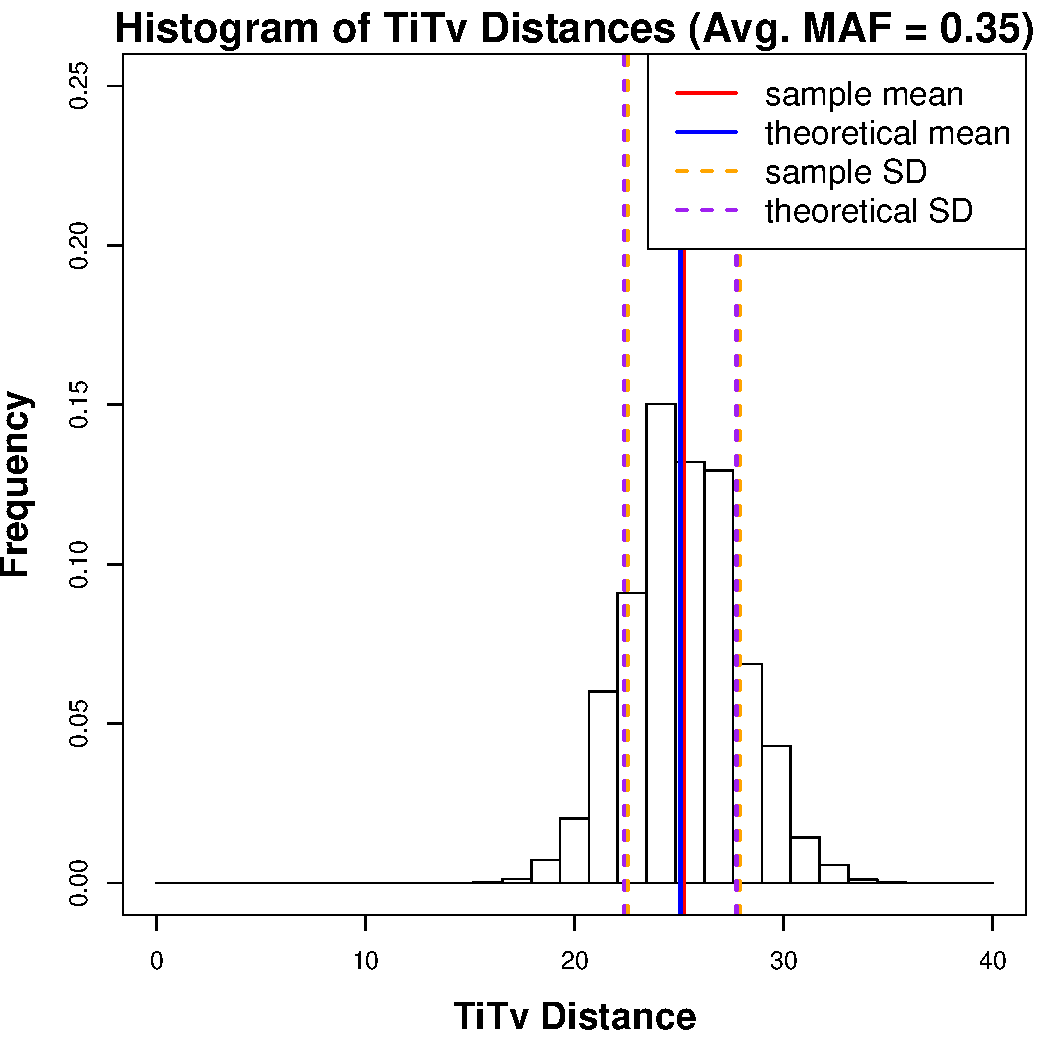
\includegraphics[width=\textwidth]{TiTv_distance_histogram_maf4.pdf}};
\node[fill=black!10,draw=black] at (10.35,-6.63) {\large \textbf{Avg. MAF} \bm{$= 0.350$}};

\node[rotate=90] at (-6.8,-5.5) {\LARGE \textbf{Density}};
\node at (7.25,-19.1) {\LARGE \textbf{TiTv Distance}};
\end{tikzpicture}

\end{document}